To evaluate the impact of our scheduler, we compare the three approaches from Section \ref{sec:scalability}. The interleaving scheduler aims to satisfy the \enquote{Optimum} solution. Additionally, we use the synchronous scheduling algorithm representing the worst case by forcing maximum interference and scheduler-less autotuning as baseline. All scenarios are considered in terms of total autotuning completion time, time for the individual stages and the resulting inference performance.

Our evaluation environment consists of two identical machines with the following specifications:
\begin{itemize}
	\item 2x Intel Xeon E5-2650 v3, 10 cores, \SI{2.30}{\giga\hertz}
	\begin{itemize}
		\item Hyper-threading enabled
		\item AVX2 instruction set
	\end{itemize}
	\item \SI{128}{\giga\byte} main memory
	\item 4x Tesla K80 \glspl{gpu}, 4992 CUDA cores, \SI{24}{\giga\byte} memory
	\item Ubuntu 16.04.6 with Linux Kernel 4.4.0
	\item Python 3.6.8
\end{itemize}

Clients always run on the first machine, while profiling servers (TVM RPC servers) always run on the second machine whose \glspl{gpu} are used as target devices. Scheduler and tracker run on the first machine to decrease network latency. They do not interfere with autotuning since they are not computationally intensive.

The number of clients and profiling servers changes for every experiment, as shown in Table \ref{tab:tvm-evaluation-setups}. On \enquote{dedicated} servers, there is only one client. Two clients run on \enquote{shared} servers. Each profiling server is assigned to a different GPU. Without interleaving, each client has its own set of four profiling servers, which might result in two servers being assigned to the same GPU. However, with interleaving, they can share the servers since they will never profile at the same time so they will not compete.
\begin{table}
	\newcommand\heading[1]{\textcolor{white}{\textbf{#1}}}
	\renewcommand{\arraystretch}{1.2}
	\sffamily
	\centering
	\begin{tabularx}{\textwidth}{l l l l X}
	\rowcolor{black} \heading{Setup} & \heading{Server~~~~~} & \heading{Scheduler~~~~~~~~~~~~~} & \heading{Bundling~~~} & \heading{Profiling servers} \vspace{2pt} \\
	\textbf{A} & Dedicated & sequential & No & 4 \\
	\textbf{B} & Shared & sequential & No & 8 \\
	\textbf{C} & Shared & synchronous & No & 8 \\
	\textbf{D} & Shared & interleaved-greedy & No & 4 \\
	\textbf{E} & Shared & interleaved-fair & No & 4 \\
	\textbf{F} & Shared & interleaved-greedy & Yes & 4 \\
	\textbf{G} & Shared & interleaved-fair & Yes & 4 \\
	\end{tabularx}
	\caption{Evaluation setups}
	\label{tab:tvm-evaluation-setups}
\end{table}

All setups are controlled by the scheduler so each experiment is affected by the---albeit minimal---overhead of scheduling and \gls{rpc}. Two separate schedulers, one for each client, are used in C to achieve natural interference. \enquote{Bundling} indicates if stages of one resource are bundled into a single stage using the \pythoninline/BundlingJobManager/, or if each stage is individually scheduled.

Our test model is a ResNet-18, which consists of 12 convolution layers and one fully connected layers, resulting in a job of 13 tasks. We autotune with 2000 trials per task and a profiling timeout of \SI{5}{\second}. Transfer learning from the global autotuning database is disabled so each experiment starts from the same, untrained cost model for a fair comparison. However, transfer learning is enabled between tasks. For time reasons, each experiment is only conducted once so the sample size is small.

A detailed chart of the autotuning times for all setups can be found in Appendix \ref{sec:results}.

\section{Results}
First, we examine the impact of interference that was qualitatively described in Section \ref{sec:scalability}. We compare A, the optimum in terms of autotuning time and inference performance, with B and C (Figure \ref{fig:chart-interference-impact}). B lets jobs naturally interfere, while C forces maximum interference as worst case scenario.\\
The baseline completion time from A is \SI{14.5}{\hour}, \SI{6.1}{\hour} (42\%) of which are spent updating the model. Natural interference results in an increase in autotuning time of \SI{4.1}{\hour} (+28\%) while forced interference takes even \SI{5.0}{\hour} (+34\%) longer\footnote{For C, the time spent waiting for the other job to finish a stage introduced by the synchronous scheduling algorithm to force interference was subtracted from the total completion time since it would not occur naturally.}. This significant increase can be attributed to slower model updates, which also experience a deterioration in performance since they are rather computationally intensive. Compared with the baseline, the total time spent updating the model increases by \SI{3.8}{\hour} (+62\%) for B and by \SI{5.2}{\hour} (+85\%) for C. Build time only increases marginally, with profiling being slightly faster, possibly due to more timeouts. B and C behave relatively similar because even without explicit scheduling, both jobs run approximately similar since they autotune the same model. In real-world scenarious with heterogenous workloads, there might be a more drastic difference.\\
The baseline inference time is \SI{48.6}{\milli\second}. B is \SI{1.5}{\milli\second} (+3\%), C is \SI{0.5}{\milli\second} (+1\%) slower. The fact that C is faster than B is probably caused by the probabilistic nature of configuration selection. The difference to the baseline is relatively small due to the large number of trials which even out the impact of interference. However, even slightly worse inference performance has a large impact with an increasing number of inferences.

\begin{figure}[ht]
	\begin{minipage}[b]{.6\textwidth}
		\centering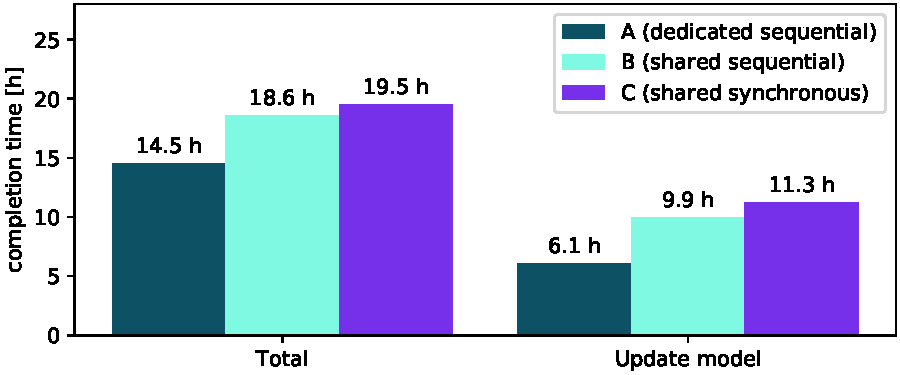
\includegraphics[width=\textwidth]{chart_interference_impact_completion}
		\subcaption{Completion time}\label{fig:chart-interference-impact-completion}
	\end{minipage}%
	\hfill
	\begin{minipage}[b]{.35\textwidth}
		\centering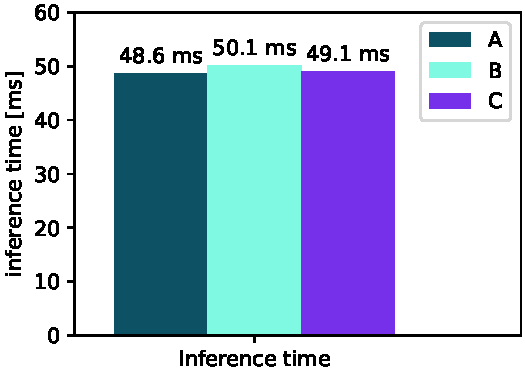
\includegraphics[width=\textwidth]{chart_interference_impact_inference}
		\subcaption{Inference performance}\label{fig:chart-interference-impact-inference}
	\end{minipage}
	\caption{Impact of interference}
	\label{fig:chart-interference-impact}
\end{figure}

We examine experiments D and E to evaluate the greedy and fair scheduler algorithm design (Figure \ref{fig:chart-interleaving}), comparing them with A as baseline. Using greedy interleaving, autotuning completes in \SI{20.4}{\hour}, \SI{5.9}{\hour} slower than A. While model update time stays about the same (\SI{0.2}{\hour} slower than A), \SI{5.5}{\hour} (27\%) of the total time is now spent waiting for resources to become free, to prevent interference. Fair interleaving is impacted even more by waiting, with total autotuning time increasing to \SI{24.1}{\hour}, \SI{9.6}{\hour} (62\%) slower than A. Model update time remains about the same (\SI{0.6}{\hour} slower than A), waiting time accumulates to \SI{8.9}{\hour} (37\% of total autotuning). Building and profiling time do not change. While the total completion time deteriorates massively, inference performance matches the baseline of \SI{48.6}{\milli\second} for both D and E because profiling interference is avoided.

\begin{figure}[ht]
	\begin{minipage}[b]{.6\textwidth}
		\centering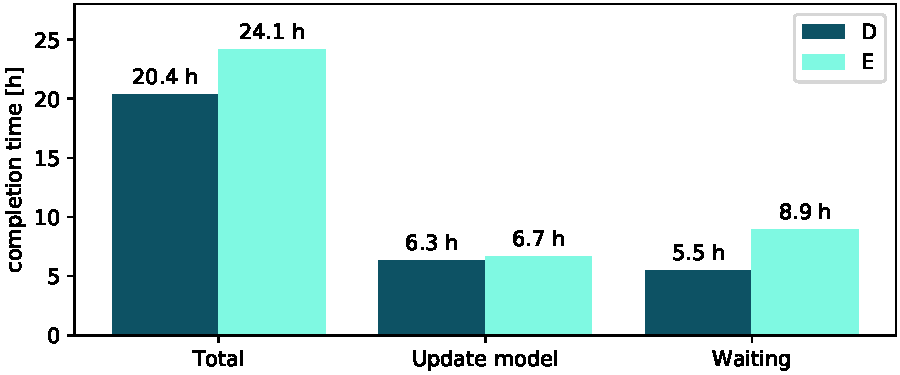
\includegraphics[width=\textwidth]{chart_interleaving_completion}
		\subcaption{Completion time}\label{fig:chart-interleaving-completion}
	\end{minipage}%
	\hfill
	\begin{minipage}[b]{.35\textwidth}
		\centering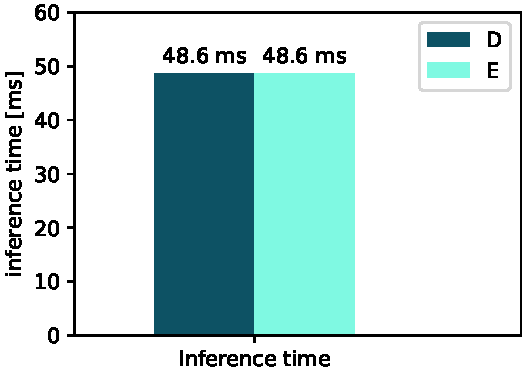
\includegraphics[width=\textwidth]{chart_interleaving_inference}
		\subcaption{Inference performance}\label{fig:chart-interleaving-inference}
	\end{minipage}
	\caption[Result of greedy versus fair interleaving]{Greedy versus fair interleaving}
	\label{fig:chart-interleaving}
\end{figure}

Finally, we examine the effect of employing bundling of stages as opposed to individually scheduling them. The greedy algorithm is used in F, the fair algorithm is used in G.
Compare to baseline and non-bundling
F already acts like batching

\begin{figure}[ht]
	\begin{minipage}[b]{.6\textwidth}
		\centering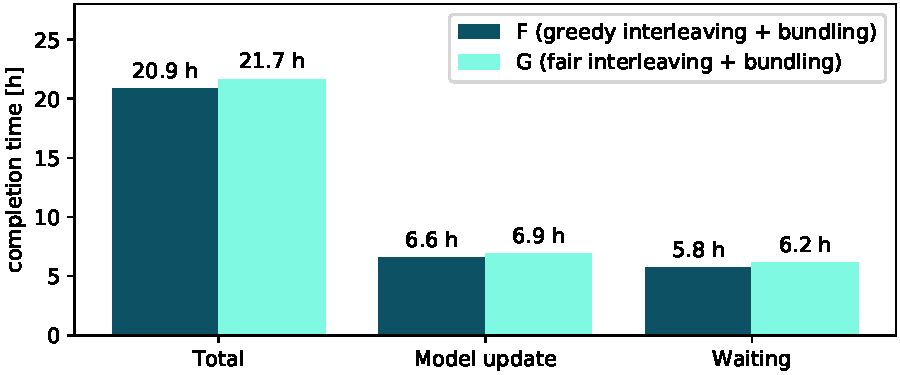
\includegraphics[width=\textwidth]{chart_bundling_completion}
		\subcaption{Completion time}\label{fig:chart-bundling-completion}
	\end{minipage}%
	\hfill
	\begin{minipage}[b]{.35\textwidth}
		\centering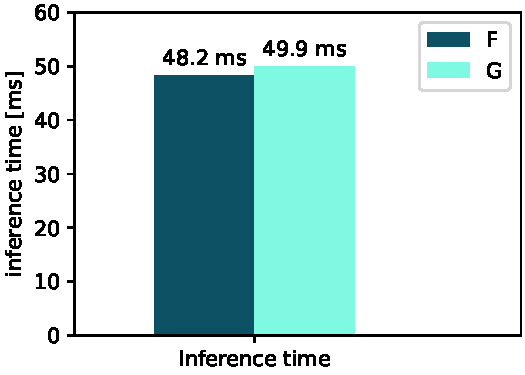
\includegraphics[width=\textwidth]{chart_bundling_inference}
		\subcaption{Inference performance}\label{fig:chart-bundling-inference}
	\end{minipage}
	\caption[Result of individual versus bundling interleaving]{Individual versus bundling interleaving}
	\label{fig:chart-bundling}
\end{figure}

\section{Discussion}
The objective of large-scale autotuning is to achieve the autotuning time and inference performance of running only a single job on each server, but with shared resources to keep the amount of required hardware at a minimum. Single-job autotuning is represented by Setup A, which is why we use it as baseline for comparisons with the other experiments.

for similar jobs on few resources: bundling
running update model and build of one job directly after another will probably decrease waiting time, since that job can then already use the target device, so there is less target device idle time
for heterogenous jobs and on larger-scale: individual interleaved provides more flexibility in combination with a more intelligent algorithm
Believe that more and heterogenous jobs that vary significantly in complexity will enable better resource utilization and less wait time, given a more intelligent scheduler

Only used scheduler for TVM, but should work for TC as well because it also has stage dependencies
greedy vs fair

Limitations:
Very rudimentary scheduler
Predictive scheduler using times for task to make scheduling more intelligent,reduce wait times
use ideas from ~\cite{Ma.2005}
Requires more control in scheduler, not only simplified interface
More sophisticated scheduler, requires moving more autotuning logic from client to scheduler
Add Knows which job is in which stage and how long is each stage estimated to take to load-awareness

The scheduler can be enhanced with more granularity for production-grade implementations.
Push instead of busy waiting

Evaluation only with limited set of hardware and models, general statement requires more experiments